% (C) Marc Lijour, 2018 
% Licensed under a Creative Commons License BY-SA
% https://creativecommons.org/licenses/by-sa/2.5/ca/
% Presentation at SIP Talks, a new series like TED Talks
%       Wake up and Smell the BlockChain!
%       Toronto: Jan 25, 2018 at 5:30 pm
% authored by Marc Lijour, January 2018
% 
% ======================================================================================================
%                                     Digital Infrastructure and Freedom
% ======================================================================================================
\section{The Freedom Gene}

\begin{frame}
	\frametitle{Settling in the New World}
	\begin{figure} % e
		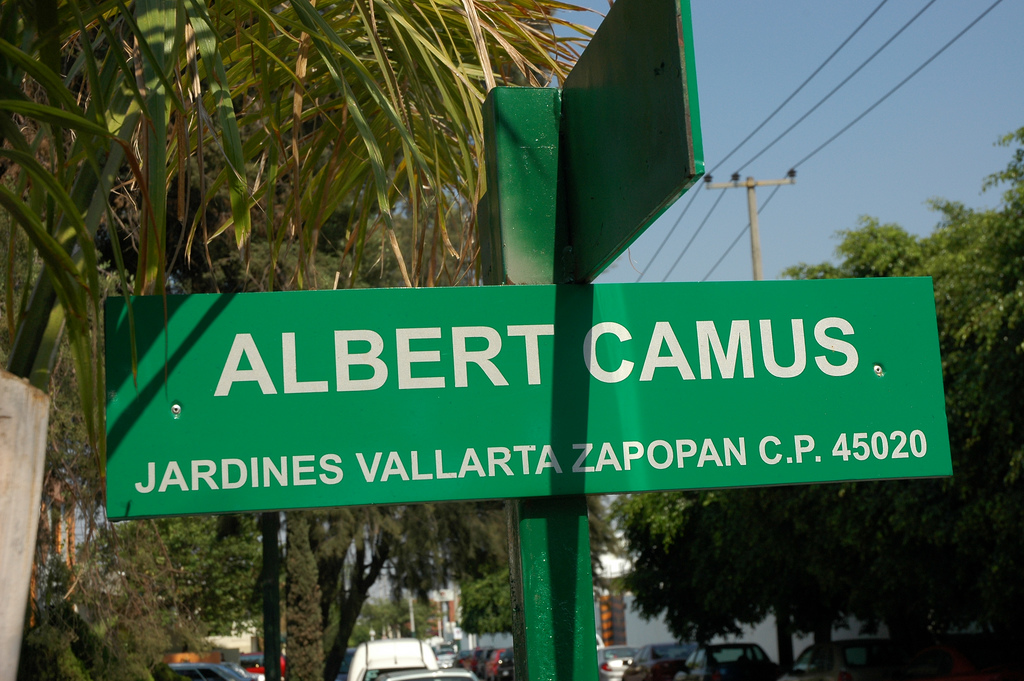
\includegraphics[width=11cm]{../pics/wonderlane2009-guadalajara_Albert_Camus}
	\end{figure}
	\tiny \copyright \href{https://www.flickr.com/photos/wonderlane/3527244519}{Wonderlane (2009)} (CC-BY license)
\end{frame}


\frame{
	\frametitle{Short History of Software}
	\framesubtitle{The birth of UNIX}
%	\framesubtitle{The birth of UNIX (Pic by Peter Hamer [\href{http://creativecommons.org/licenses/by-sa/2.0}{CC BY-SA 2.0}], via Wikimedia Commons)}
	\begin{figure}
	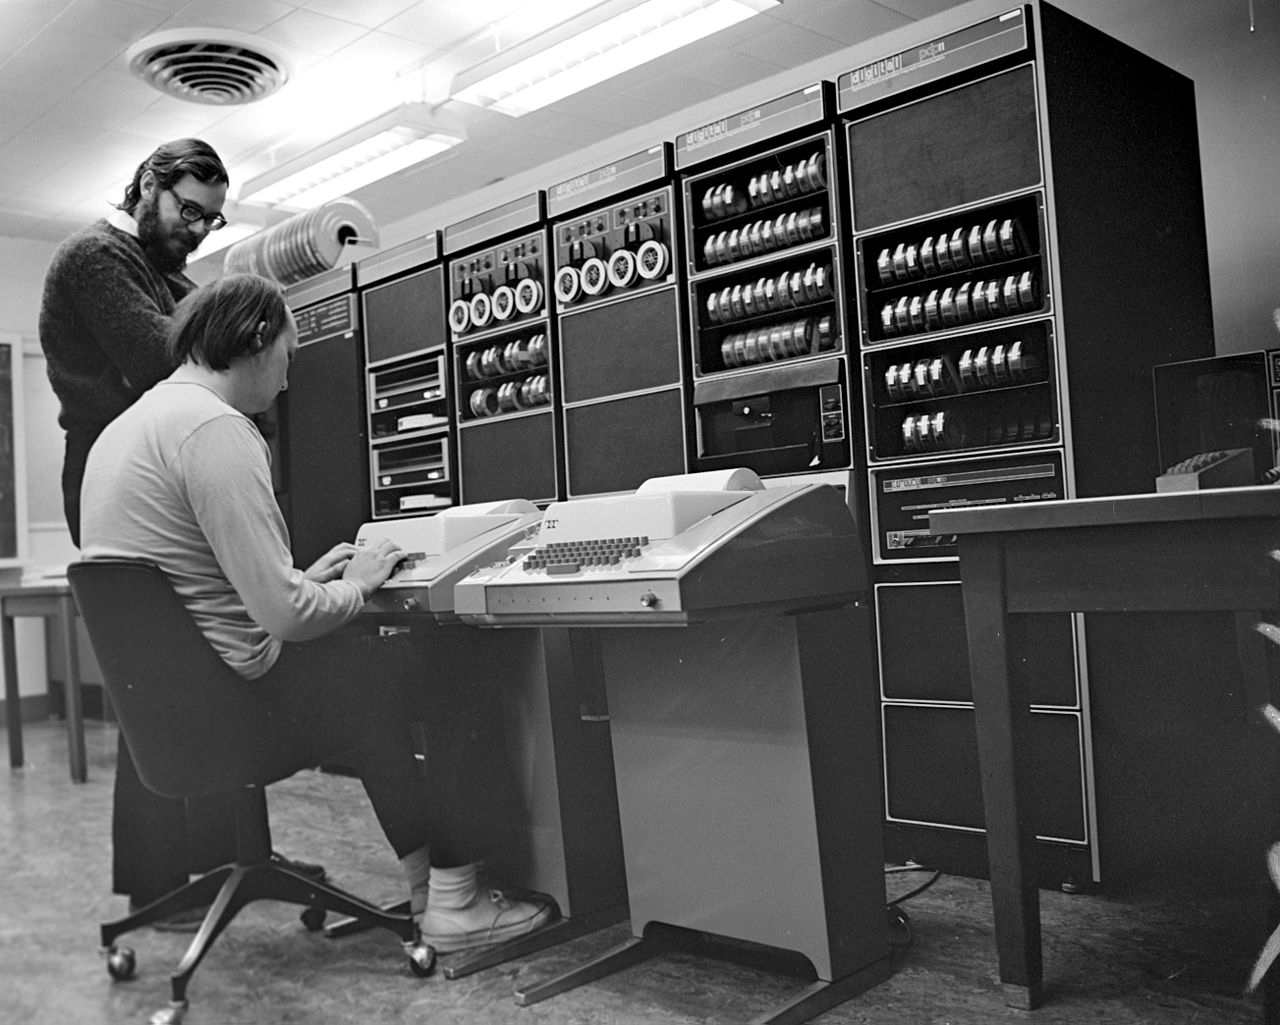
\includegraphics[height=6.4cm]{../pics/Ken_Thompson_(sitting)_and_Dennis_Ritchie_at_PDP-11_(2876612463)}
	\caption{Ken Thompson (sitting) and Dennis Ritchie at PDP-11}
	\end{figure}
	\tiny \copyright \href{http://creativecommons.org/licenses/by-sa/2.0}{Peter Hamer} (CC BY-SA 2.0 license)
}

\begin{frame}
	\frametitle{Free Software}
	\begin{figure}
		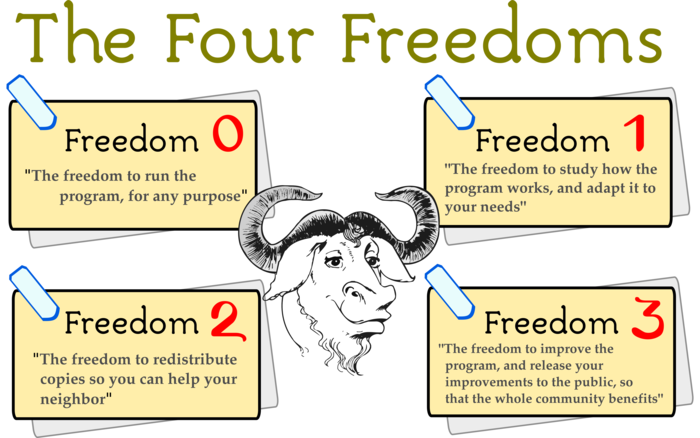
\includegraphics[width=11cm]{../pics/scaled_full_00c40105cea4c0aa3e9f}
	\end{figure}
\end{frame}


\frame{
	\frametitle{Free Software and Open Source Software}
%	\framesubtitle{An introduction to Free/Libre Open Source Software (\href{https://www.youtube.com/watch?v=Tyd0FO0tko8}{Intel, 2014})}
	\framesubtitle{An introduction to Free/Libre Open Source Software (\cite{intel2014:FLOSS})}
	\begin{figure}
	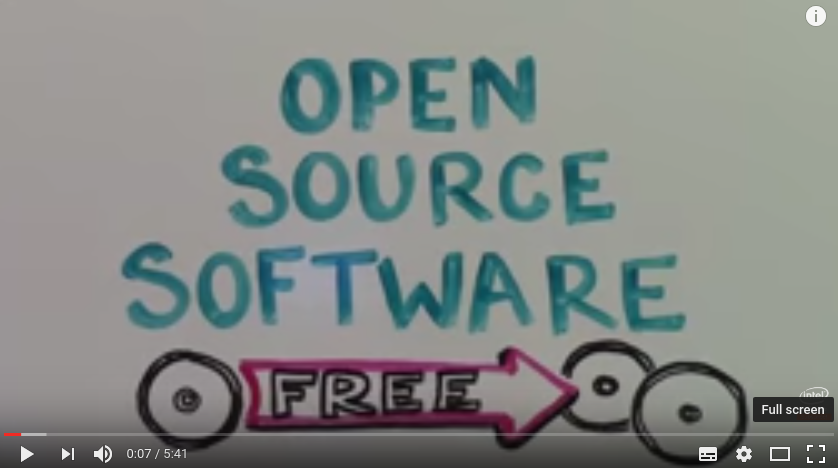
\includegraphics[height=5cm]{../pics/intel-FLOSS-intro}
	\caption{\url{https://www.youtube.com/watch?v=Tyd0FO0tko8}}
	\end{figure}
	\tiny \copyright \href{https://www.youtube.com/watch?v=Tyd0FO0tko8}{Intel Software (2014)}
}

\begin{frame}
	\frametitle{Open Source runs (almost) Everything}
	\framesubtitle{2015 was an inflexion point}
	\begin{figure} % extracts from articles and other sources published on the Web
		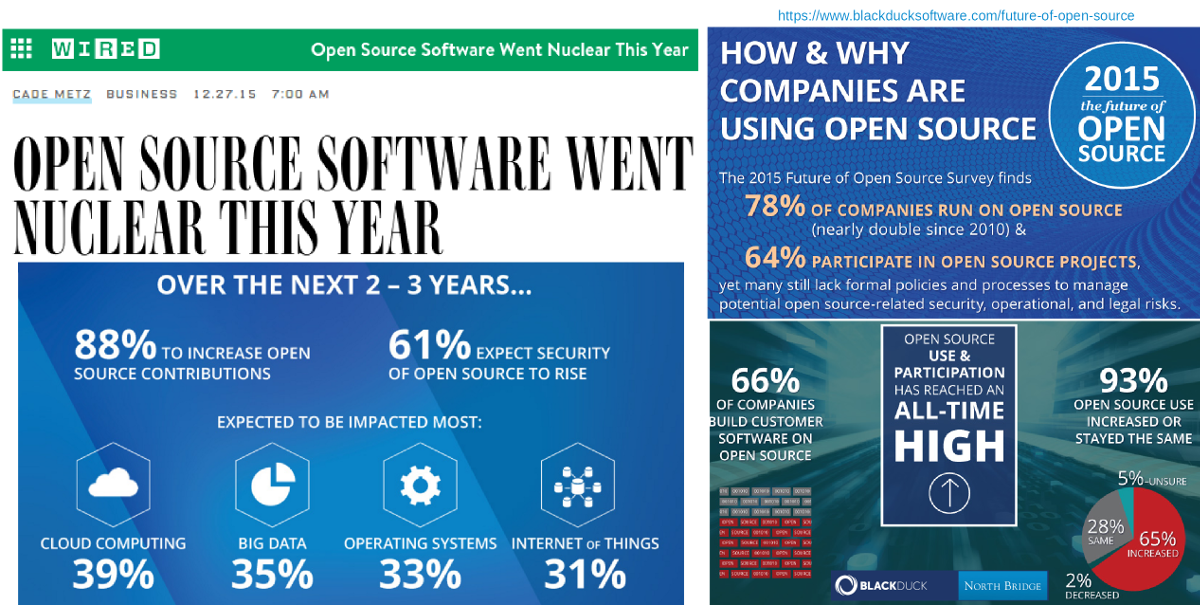
\includegraphics[width=11cm]{../pics/pic-open-source-went-nuclear-non-interlaced}
	\end{figure}
\end{frame}

\frame{
	\frametitle{From IoT to Cloud and AI, and of course Blockchain}
	\begin{figure}
	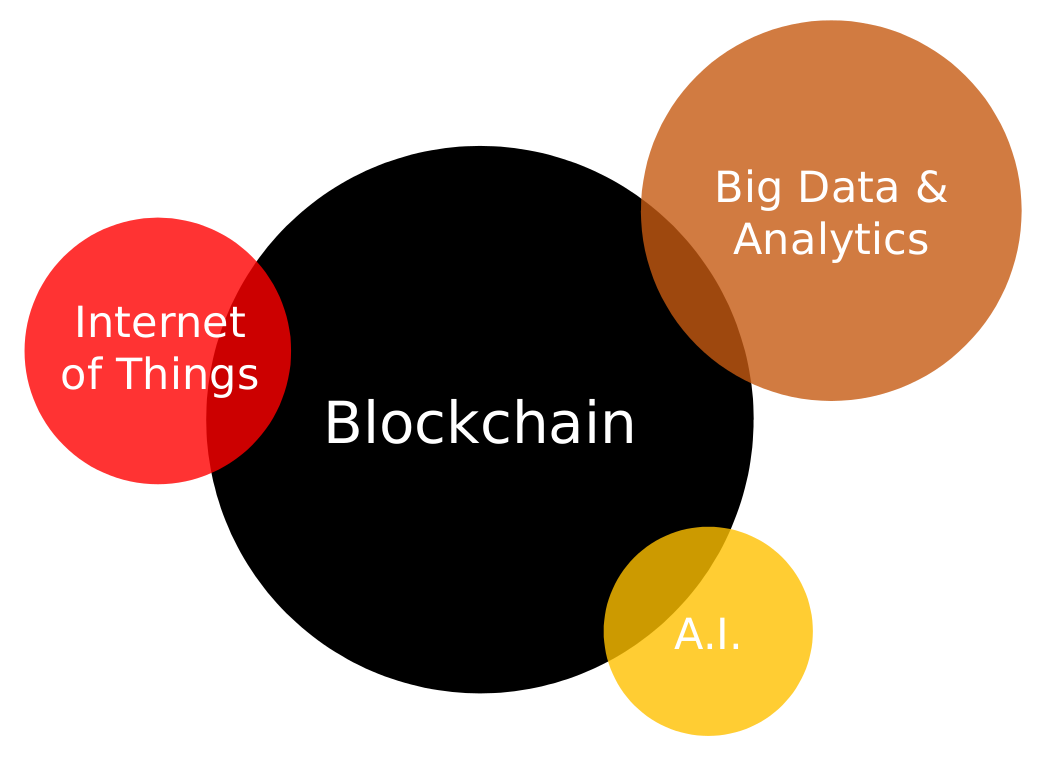
\includegraphics[width=10cm]{../../pics/colliderx/blockchain-plus-AI-etc}
	\end{figure}
}

\frame{
	\frametitle{The Milenials}
	\begin{figure} % https://www.flickr.com/photos/statefarm/26663820390
		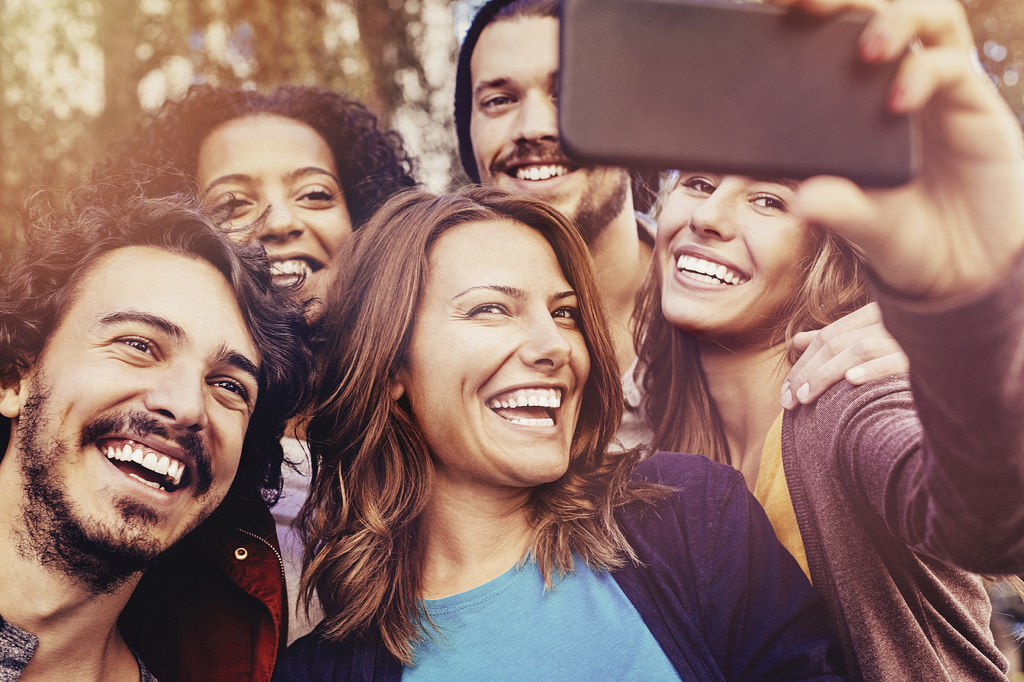
\includegraphics[width=11cm]{../pics/statefarm-milenials-CC-BY}
	\end{figure}
	\tiny \copyright \href{https://www.flickr.com/photos/statefarm/26663820390}{State Farm} (CC-BY license)
}

\frame{
	\begin{block}{}
		\begin{quote}
			{\Huge 20\% of the world's economy will be digital by 2020.} \\
			\vspace{1em}
			\hfill ---Accenture \#techvision2016
		\end{quote}
	\end{block}
}


% ======================================================================================================
%                                     Difficulty to Fund the Commons
% ======================================================================================================
\section{The Tragedy of the Commons}

\frame{
	\frametitle{The Tragedy of the Commons}
	\begin{figure}
	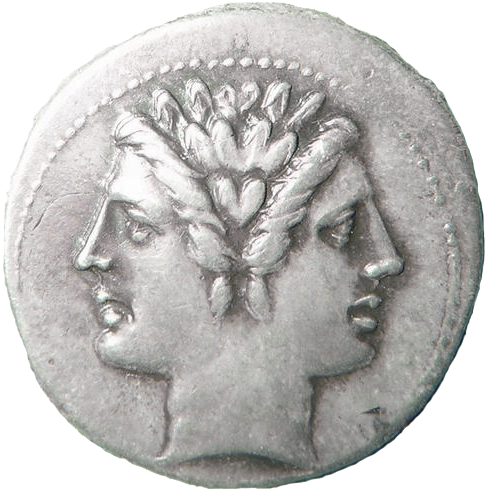
\includegraphics[width=6cm]{../pics/janus_coin}
	\end{figure}
}

\frame{
	\frametitle{Nadia Eghbal's report (\citeyear{eghbal2016})}
	\framesubtitle{Roads and Bridges: The Unseen Labor Behind Our Digital Infrastructure}
	\begin{columns}
	\column{0.3\textwidth}
		\begin{figure}
		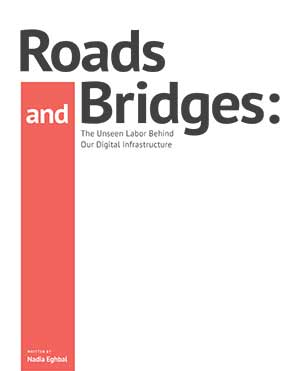
\includegraphics[width=3cm]{../pics/logos/roads-and-bridges}
		\end{figure}
	\column{0.7\textwidth}
	\begin{itemize}
        \item Open Source Software runs core infrastructure services
        \item It is poorly funded (e.g. OpenSSL)
        \item Who should fund roads and bridges?
    \end{itemize}
	\end{columns}
}

\frame{
	\frametitle{Other issues}
	\begin{itemize}
        \item Ability (and need) to run software to open archived files
        \pause
        \item Deletion or lack of back-ups\\
            {\small \emph{(in 1999, 40\% of companies had lost or thrown away the source code of their systems)}}
        \pause
        \item Project shutdown (e.g. Google Code circa 2014)
        \pause
        \item Repository taken hostage (e.g. Code Spaces) % https://www.infoworld.com/article/2608076/data-center/murder-in-the-amazon-cloud.html
        \pause
        \item The half-life of an URL is about 4 years
    \end{itemize}
}

\frame{
	\frametitle{The universal software archive}
    \framesubtitle{https://www.softwareheritage.org}
	\begin{figure}
	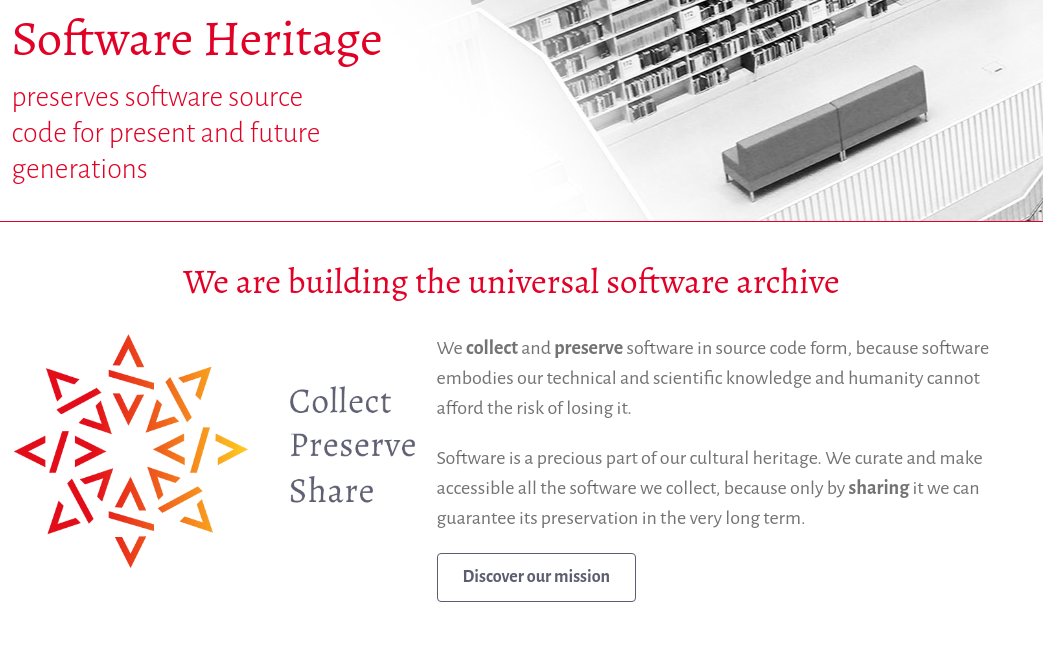
\includegraphics[width=10cm]{../pics/software_heritage}
	\end{figure}
}

\frame{
	\frametitle{Basic Tips to fund Free/Libre Open Source Software}
    \framesubtitle{see also Nadia Eghbal (\citeyear{eghbal:funding})}
	\begin{itemize}
        \item Individual Time
        \pause
        \item Community support (tee-shirt sales, ads, DVD burning, donations)
        \pause
        \item Corporate investment
        \pause
        \item Sales (licensing)
        \pause
        \item Large Donations and Grants
    \end{itemize}
}


% 
% ======================================================================================================
%                                     ColliderX
% ======================================================================================================
\section{ColliderX: the world-first crowdfunded R\&D Hub focusing on Blockchain and related technologies}

\frame{
	\frametitle{\citeauthor{colliderx}} %ColliderX
	\framesubtitle{\url{https://www.collider-x.org}}
	\begin{itemize}
		\item World-first Open Source Crowdfunded R\&D Hub focusing on Blockchain and related technologies (AI, IoT, ...)
		\pause
		\item Building \href{http://www3.weforum.org/docs/WEF_Realizing_Potential_Blockchain.pdf}{the digital infrastructure of tomorrow}
		\pause
		\item Now building a Blockchain \href{https://www.ic.gc.ca/eic/site/093.nsf/eng/00003.html}{Innovation Supercluster} in Canada
		\pause
		\item Open to all researchers/developers/tinkerers and backers in the world
	\end{itemize}
}

\frame{
	\frametitle{Starting your own Free/Libre Open Source Software project}
    \framesubtitle{Nicely summarized by Roberto Di~Cosmo (\citeyear{dicosmo:achieving-impact})}
	\begin{itemize}
        \item Identify a need
        \pause
        \item Build a prototype
        \pause
        \item Grow a community
        \pause
        \item Set up an ecosystem (users, developers, architects, designers, service providers...)
% the last two are the most difficult
    \end{itemize}
}

\frame{
	\frametitle{How to engage with ColliderX?}
	\begin{itemize}
        \item Backers
        \item Researchers/Developers
    \end{itemize}
}



